\documentclass[aspectratio=169]{beamer}
\usepackage[utf8]{inputenc}
\usepackage[T1]{fontenc}
\usepackage{listings}

\usetheme{Madrid}
\usecolortheme{default}

%------------------------------------------------------------
\title[MapReduce]
{Hadoop MapReduce}

\author[Claudio, Gabriell]
{Claudio~Scheer\inst{1} \and Gabriell~Araujo\inst{1}}

\institute[PUCRS]
{
	\inst{1}
	Master's Degree in Computer Science\\
	Pontifical Catholic University of Rio Grande do Sul - PUCRS
}

\date[2020]
{High Performance for Big Data Applications}
%------------------------------------------------------------

%------------------------------------------------------------
\AtBeginSection[]
{
	\begin{frame}
		\frametitle{Table of Contents}

		\tableofcontents[currentsection]
	\end{frame}
}
%------------------------------------------------------------

\begin{document}

\frame{\titlepage}

%---------------------------------------------------------
\begin{frame}
	\frametitle{Table of Contents}

	\tableofcontents
\end{frame}
%---------------------------------------------------------

%---------------------------------------------------------
\section{Hadoop}

\begin{frame}
	\frametitle{What we mean by Hadoop}

	\begin{center}
		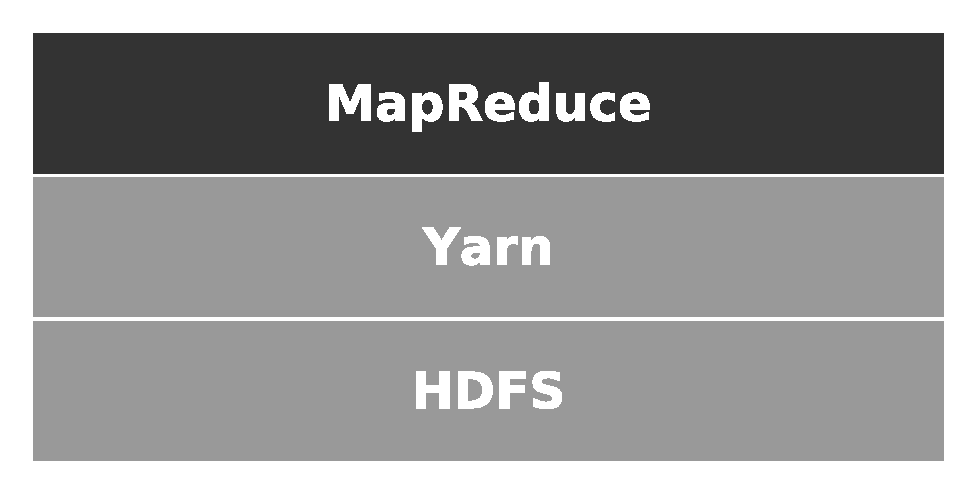
\includegraphics[height=1\textheight,width=0.6\textwidth,keepaspectratio]{./images/hadoop.pdf}
		{\tiny \href{https://data-flair.training/blogs/hadoop-ecosystem-components}{https://data-flair.training/blogs/hadoop-ecosystem-components}}
	\end{center}
\end{frame}

\begin{frame}
	\frametitle{MapReduce execution flow}

	\begin{center}
		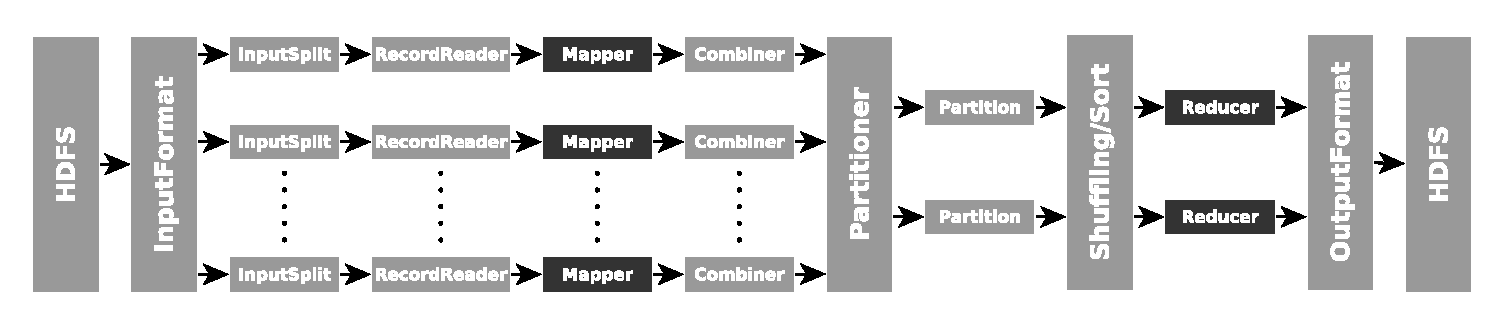
\includegraphics[height=1\textheight,width=1\textwidth,keepaspectratio]{./images/map-reduce.pdf}
		{\tiny \href{https://data-flair.training/blogs/hadoop-ecosystem-components}{https://data-flair.training/blogs/hadoop-ecosystem-components}}
	\end{center}
\end{frame}

\begin{frame}[fragile]
	\frametitle{Custom data types}

	\begin{columns}
		\column{0.4\textwidth}
		\begin{itemize}
			\item LongWritable = long;
			\item IntWritable = int;
			\item Text = String;
			\item \href{https://hadoop.apache.org/docs/current/api/org/apache/hadoop/io/package-summary.html}{Other data types (link);}
		\end{itemize}


		\column{0.6\textwidth}
		\begin{lstlisting}[language=java,basicstyle=\tiny,columns=fullflexible]
public class IntWritable implements WritableComparable<IntWritable> {
  private int value;

  public IntWritable(int value) { set(value); }

  public void set(int value) { this.value = value; }

  public int get() { return value; }

  @Override
  public void readFields(DataInput in) throws IOException {
    value = in.readInt();
  }

  @Override
  public void write(DataOutput out) throws IOException {
    out.writeInt(value);
  }

  @Override
  public int compareTo(IntWritable o) {
    int thisValue = this.value;
    int thatValue = o.value;
    return (thisValue < thatValue ? -1 : (thisValue == thatValue ? 0 : 1));
  }
}
        \end{lstlisting}
		{\tiny \href{https://github.com/apache/hadoop/blob/master/hadoop-common-project/hadoop-common/src/main/java/org/apache/hadoop/io/IntWritable.java}{\beamergotobutton{Source}}}
	\end{columns}
\end{frame}

\begin{frame}
	\frametitle{InputFormat}

	\begin{itemize}
		\item TextInputFormat: <LongWritable, Text>
		\item KeyValueTextInputFormat: <Text, Text>
		      \begin{itemize}
			      \item Key splitted by \textbackslash t;
		      \end{itemize}
		\item NLineInputFormat: <LongWritable, Text>
		      \begin{itemize}
			      \item {\scriptsize \texttt{config.setInt(``mapreduce.input.lineinputformat.linespermap'', 10000)}};
		      \end{itemize}
		\item Customs InputFormat must implement \texttt{getSplits} and \texttt{getRecordReader};
		      \begin{itemize}
			      \item {\tiny \href{https://hadoop.apache.org/docs/stable/api/org/apache/hadoop/mapred/InputFormat.html}{https://hadoop.apache.org/docs/stable/api/org/apache/hadoop/mapred/InputFormat.html}}
		      \end{itemize}
	\end{itemize}
\end{frame}

\begin{frame}
	\frametitle{InputSplit}

	\begin{itemize}
		\item Defines the parallelism level;
		\item Usually splitted by the size of the block;
		      \begin{itemize}
			      \item 10TB/128MB = 82000
		      \end{itemize}
		\item It is a logical division of the input data;
		\item Ways to change it:
		      \begin{itemize}
			      \item {\scriptsize \texttt{config.set(MRJobConfig.NUM\_MAPS, 2)}};
			      \item {\scriptsize \texttt{mapreduce.job.maps} on \texttt{mapsite-site.xml}};
		      \end{itemize}
	\end{itemize}

	\begin{center}
		{\tiny \href{https://hadoop.apache.org/docs/current/hadoop-mapreduce-client/hadoop-mapreduce-client-core/MapReduceTutorial.html}{https://hadoop.apache.org/docs/current/hadoop-mapreduce-client/hadoop-mapreduce-client-core/MapReduceTutorial.html}}
	\end{center}
\end{frame}

\begin{frame}[fragile]
	\frametitle{RecordReader}

	\begin{itemize}
		\item Split InputSplit into <key, value> pairs;
		      \begin{itemize}
			      \item Custom implementations can read values from outside the InputSplit;
		      \end{itemize}
		\item Max record length:
		      \begin{itemize}
			      \item {\scriptsize \texttt{config.setInt(``mapreduce.input.linerecordreader.line.maxlength'', Integer.MAX\_VALUE);}}
		      \end{itemize}
		\item Vanilla example:
		      \begin{lstlisting}[language=java,basicstyle=\tiny,columns=fullflexible]
        run(Context context) {
            while(context.nextKeyValue())
            {
                map(context.setCurrentKey(), context.getCurrentValue(), context)
            }
        }
            \end{lstlisting}
	\end{itemize}
\end{frame}

\begin{frame}
	\frametitle{Mapper}

	\begin{itemize}
		\item Maps <key1, value1> to <key2, value2>;
	\end{itemize}
\end{frame}

\begin{frame}
	\frametitle{Combiner}

	\begin{itemize}
		\item Reduces data transfer between mapper and reducer;
		\item Reduces the amount of data to be processed in the reducer;
	\end{itemize}

	\begin{center}
		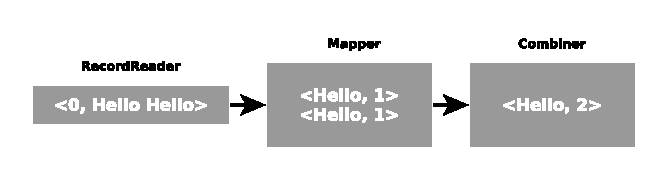
\includegraphics[height=1\textheight,width=0.8\textwidth,keepaspectratio]{./images/combiner.pdf}
	\end{center}
\end{frame}
%---------------------------------------------------------

%---------------------------------------------------------
\section{Examples}

- WordCount;
- CountProductsSold;
-

\begin{frame}
	\frametitle{Sample frame title}

	In this slide, some important text will be
	\alert{highlighted} because it's important.
	Please, don't abuse it.

	\begin{block}{Remark}
		Sample text
	\end{block}

	\begin{alertblock}{Important theorem}
		Sample text in red box
	\end{alertblock}

	\begin{examples}
		Sample text in green box. The title of the block is ``Examples".
	\end{examples}
\end{frame}

\begin{frame}
	\frametitle{Two-column slide}

	\begin{columns}

		\column{0.5\textwidth}
		This is a text in first column.
		$$E=mc^2$$
		\begin{itemize}
			\item First item
			\item Second item
		\end{itemize}

		\column{0.5\textwidth}
		This text will be in the second column
		and on a second tought this is a nice looking
		layout in some cases.
	\end{columns}
\end{frame}
%---------------------------------------------------------


\end{document}
